\clearpage
\section{Initial Chunk Size}
\label{sec:evaluation-initial-chunk}

\begin{figure*}[!htb]
	\begin{minipage}[t]{0.8\linewidth}
	\begin{center}
      	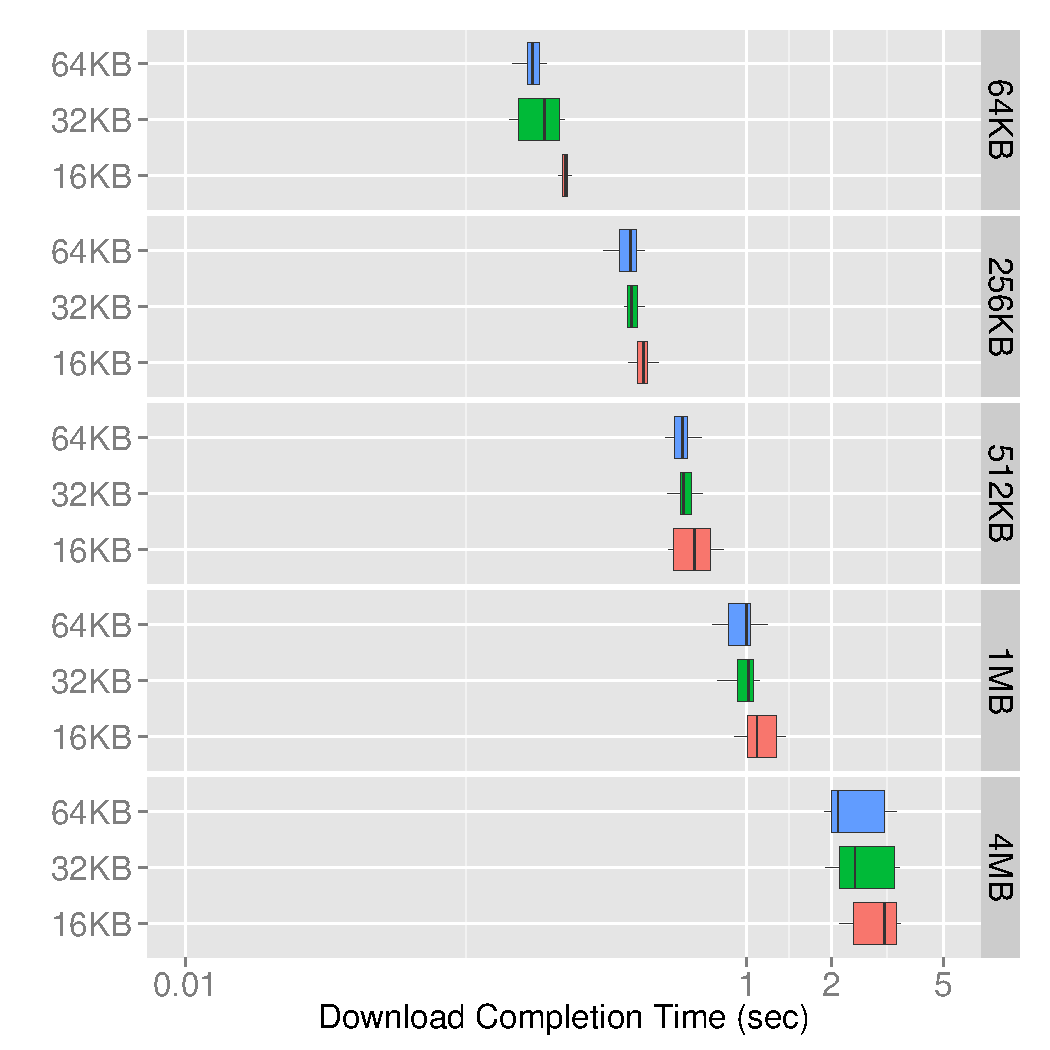
\includegraphics[width=\linewidth]{Figures/dynamic-alpha-initial-chunk.pdf}
		\caption{\label{fig:evaluation-initial-chunk-alpha} Effect of initial chunk size on \algalpha.}
    \end{center}
	\end{minipage}
\vspace*{-0.3cm}
\end{figure*}
\begin{figure*}[!htb]
    \begin{minipage}[t]{0.8\linewidth}
    \begin{center}
        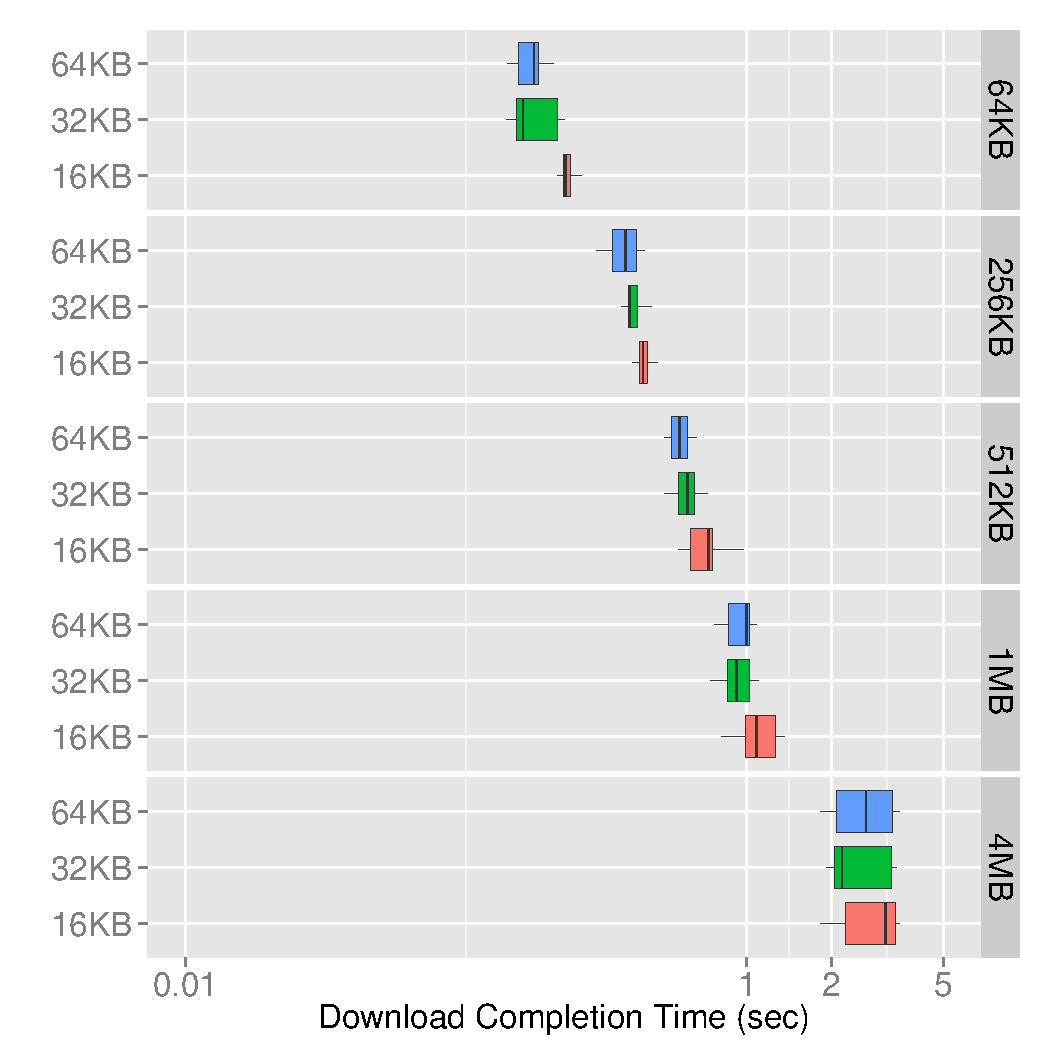
\includegraphics[width=\linewidth]{Figures/dynamic-slice-initial-chunk.pdf}
      	\caption{\label{fig:evaluation-initial-chunk-slice} Effect of initial chunk size on \algslice.}
    \end{center}
    \end{minipage}
  \vspace*{-0.3cm}
\end{figure*}

%- 16KB performs worse, 16KB might not be enough to get a good first link estimate, resulting in small chunks, thus more request overhead

%- 32KB and 64KB seem to perform similar

%- similar results in both schedulers - initial chunk size seems to have same effect

%- be careful in case of website downloads

%- explain that we use 32K initial chunk size (similar like in paper)

We study the effect of the initial chunk size on the \algalpha~and the \algslice~algorithm. 
We take the download completion time as the major metric. 
We measure over $30$ rounds, with each round having a randomized configuration sequence in order to account for traffic dependencies and/or correlation. 
We depict the median, $25-75$\perc percentiles (boxes), and the dispersion (lines, $5-95$\perc percentiles). 
In~\fref{fig:evaluation-initial-chunk-alpha} and~\fref{fig:evaluation-initial-chunk-slice} we see the results for 3 different chunk sizes, \ie $16$KB, $32$KB and $64$KB for \algalpha~and \algslice~respectively. 
The initial chunk size of $16$KB tends to perform worse than initial chunk sizes of $32$KB or $64$KB. 
This is expected; since a small initial chunk could increase the total amount of requests necessary to download a file, which consequently leads to a higher request overhead. 
Moreover, when using very small initial chunks there is a higher chance that the link quality estimate is not very accurate, which might result in bad scheduling decisions for the first chunks. 

We further see that a chunk size of $64$KB tends to perform best, especially on $64$KB files. 
This is reasonable, since the file is downloaded in a single request, whereas with a $32$KB initial chunk a further request is necessary. 
Even when using a second connection, a certain time is necessary to establish that connection. 
This plus the extra request overhead explain the loss compared to $64$KB initial chunks. 

It is important to note that we do not know the link quality prior to an initial chunk request, meaning that in case of a bad link choice a high initial chunk size might be harmful since the initial chunk needs to be downloaded over that link. 
Only after downloading the initial chunk, we obtain information about the link quality to make intelligent chunk size decisions. 
Due to this, we set the initial chunk size to an intermediate value of $32$KB as a compromise between the benefits and the risks. 
Note, that this is an arbitrary choice and further study is necessary to determine the optimal initial chunk size. 
